\begin{comment}
Based upon current SOTA ensemble methods is common practice to improve generalisation of a system.
As shown in results of COCO, resolution of an object in an image a major factor in performance.
Another issue not often discussed in works is image quality. Can be a factor in performance - cite IQDNN paper
Different methods to tackle this problem. 
for resolution, dependent on two parts of the the object detector, 1. object proposals 2. classification of proposals
	if proposals have a low recall then classification part of detector is never presented with objects and no way to classify them
	if classification is poor then cannot classify.....
possible to create an ensemble for either, chosen to concentrate on the latter

plan
address pillars 1 and 3 of an ensemble system
1 - train on different subsets of data
previous works have done this randomly and tested on a validation set
here, instead actively create different subsets to train on and to test on
3 - ensemble detections of above models
majority, dynamic, etc

present method as to how to measure image quality
what is FR IQA / NR IQA?

show figure of how to ensemble

choice of ResNet-101 GPU size
\end{comment}

\section{Design Overview}
Now that an analysis of the technical aspects of object detection with deep learning has been conducted an overview of the design of the system will be made in this section. 
Multiple choices can be made with respect to the overall architecture of the \gls{cnn}-based object detector. As covered in \sectionref{objdet}, two of the best performing systems are Faster R-CNN and R-FCN. Both methods have similarities in their overall architecture. Such as taking advantage of an \gls{rpn} to efficiently find region proposals. Additionally the current core classification model used in both is the ResNet architecture. As the addition of ResNets significantly increases performance the use of these in this work is deemed as crucial part. However, the choice of either Faster R-CNN or R-FCN is not immediately as clear. Both methods perform similarly with respect to benchmarks such as \gls{pascalvoc} and \gls{mscoco}. However, as the decision has been made to incorporate ResNets a decision on this matter was indirectly made. The GPU available in this project while being large in regards to memory was only available to train R-FCN with the ResNet-101 model. Unfortunately, due to the internal architecture of Faster R-CNN the 8Gb memory on the NVIDIA GPU was not able to store all parameters while training a Faster R-CNN with ResNets. However, due to the more efficient classification module in R-FCN, a ResNet backbone could be trained.
\\\\
As mentioned, leading object detection systems take advantage of ensemble methods. However, many of them are trained with regards to the internal architecture and not specifically training experts towards solving specific challenges. Therefore, the system in this project will take advantage of the first point in \sectionref{build_ensemble}, namely data sampling and selection. The aim will be to train R-FCN with ResNet-101 on different subsets of training data with the aim to create expert ensemble members in regards to factors present. Two separate factors will be chosen, one with respect to variations in the object and the other in terms of image variations. The first factor chosen in object size, as seen in \sectionref{benchresults}, in general object detection systems find it challenging to detect and classify smaller objects. Therefore, if a system can be trained towards a subset of sizes in the training data, ideally the individual ensemble members will increase their performance on the respective sizes. The second factor chosen is in with image quality. As mentioned in \sectionref{qualityprob}, the quality of an image can be a factor in the overall performance of \gls{cnn}-based classification systems. Therefore members will also be trained towards subsets data split based upon this.
Lastly, individual members predictions much be combined in an ensemble system. Therefore, approaches must be taken to combine outputs. The combination strategy is greater than only voting on which class a potential object is associated to. Bounding-boxes and the confidence of each detection is used in the calculation of metrics in both \gls{pascalvoc} and \gls{mscoco}. Therefore these must be combined in the ensemble system as well.
\\\\
Based upon these issues the following design requirements are set with respect to the previously discussed items.

\begin{itemize}
	
	\item Object Detector Architecture.
	\begin{itemize}
		\item \gls{cnn}-based method.
		\item ResNets as backbone model.
	\end{itemize}

	\item Ensemble Data Sampling and Selection.
	\begin{itemize}
		\item Ability to measure object and image variations with respect to: 
		\begin{itemize}
			\item Object size.
			\item Image Quality.
		\end{itemize}
	\end{itemize}

	\item Ensemble Training of Classifiers.
	\begin{itemize}
		\item Must be kept constant to measure effect of differing data sampling strategies.
	\end{itemize}

	\item Ensemble Combination.
	\begin{itemize}
		\item Method to combine individual bounding-boxes and confidences between individual ensemble members.
	\end{itemize}
\end{itemize}

Now that the general requirements have been outlined the following sections will cover the architectural considerations to ensure that the above requirements can be met.

\subsection{Training R-FCN}
The training of the R-FCN object detectors will be done in the \gls{caffe} \cite{caffe}. This was chosen due to the research being provided by the authors of R-FCN through training code and pre-trained \gls{caffe} models. However, as there is the requirement mentioned in the previous section, that in order to combine detections between ensemble members the detection must be found based upon the same input to the model. One solution to this is to use the region proposals found using the R-FCN's \gls{rpn}. In a standard R-FCN the \gls{rpn} is an internal part of the network and is trained end-to-end. However, as these proposals must be constant between all ensemble members this method is not appropriate. Additionally, due to the nature of the \gls{caffe} framework, once a network has been defined and trained it is difficult to change it. For example, a standard R-FCN takes the entire image as inputs but in this work the requirement is that it takes smaller region proposals. The solution to these points is to train the networks using a method inspired by the 4-step alternating training method presented by the Faster R-CNN authors \cite{fasterrcnn}. The process can be seen in \figref{4steptrain}.

 \begin{figure}[H]
  \centering
    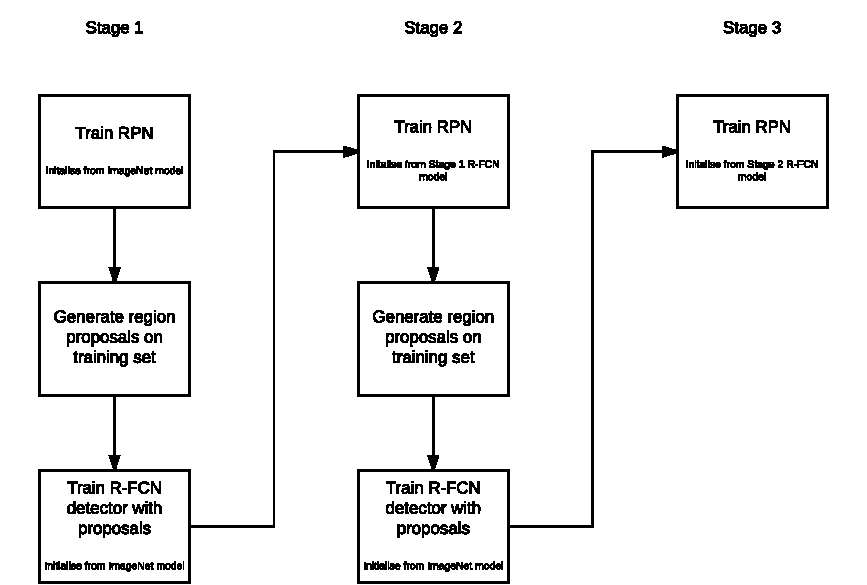
\includegraphics[width=1.0\textwidth]{Figs/Design/4steptrain1.pdf}
      \caption{Flow chart showing the 4-step alternating training method.}
    \label{fig:4steptrain}
\end{figure}

In this approach the overall network in trained in multiple steps rather than an end-to-end method. In the first step a \gls{rpn} is trained to determine region proposals, the \gls{rpn} is initialised from a pre-trained ImageNet model and fine-tuned to the proposal task. Next a \gls{rfcn} is trained based upon the proposals found in the previous step. This network is also initialised with a pre-trained ImageNet model. In step three, another \gls{rpn} is trained but initialised using the \gls{rfcn} from step two. In this step the convolutional layers that are shared between the \gls{rfcn} and \gls{rpn} are fixed and only the layers unique to the \gls{rpn} are updated. By training a model with this approach a testing image is able to run through the same steps as a \gls{rfcn} trained end-to-end, however, as the networks are split into different models it is also possible to use the stages of the method individually. Creating a solution for finding region proposals with an \gls{rpn} and having a \gls{rfcn} that can take the proposals as inputs. 
\\\\
An additional benefit to training \glspl{rfcn} in this manner is that as the aim is to train ensemble members to different subsets of data, once a baseline model has been created only one part needs to be re-trained. This being the final step in stage 2, training the R-FCN detector. The \gls{rpn} in stage 3 should be kept constant based on the baseline model as it will provide the shared proposals for test images. Therefore, once a systematic approach has been found for splitting data for both train and test based on the data sampling and selection requirements the detection part of the \gls{rfcn} can be trained towards its expert area. The following sections will explain how the subsets of data will be selected.

\subsubsection{Object Size Training}
The area of a region proposal gives an indication as to the approximate size of a potential objects. Therefore, the area for all proposals on the training set can be computed from the output of the second step in stage 2 shown in \figref{4steptrain}. Once computing the area of all proposals an appropriate split of the data can be determined depending on the distribution for the given training data set. The main requirement in creating the subsets of data is that equal number of ground truth samples should be present in both.

\subsubsection{Image Quality Training}
There are many choices for computing the quality of an image. A popular area of research for this purpose is \gls{iqa}. These methods aim to determine the subjective quality of an image. There are two popular forms of \gls{iqa}, \gls{friqa} and \gls{nriqa}. \gls{rfiqa} approaches require the original, undistorted reference image in order to determine quality. Whereas, \gls{nriqa} do not have this information available. As the aim is to determine quality on
